\documentclass[11pt,letterpaper]{article}

\usepackage{geometry}
\geometry{margin=1in}

\usepackage{graphicx}
\usepackage{float}
\usepackage{subcaption}
\usepackage{booktabs}

% paragraph formatting
\setlength{\parindent}{0pt}
\setlength{\parskip}{0.5em}

% make lists tighter
\usepackage{enumitem}
\setlist{nolistsep}

% reduce spacing before and after section
\usepackage{titlesec}
\titlespacing\section{0pt}{6pt}{0pt}

\title{Lab 1 - PECARN TBI Data, STAT 215A, Fall 2026}

\begin{document}

\maketitle

\section{Introduction}\label{introduction}

Traumatic brain injury (TBI) is a leading cause of death and disability among children. 
Computed tomography (CT) is the primary method used by physicians to identify traumatic brain injuries
following head injury. However, CT scans expose children to ionizing radiation, which is 
associated with an increased lifetime risk of lethal malignancy (i.e., cancer).
Physicians must therefore weigh the immediate benefit of CT for identifying a
clinically imporant traumatic brain injury (ciTBI) against the potential long-term
risks from radiation exposure. As CT use has increased, developing reliable decision rules
within the context of this trade-off has become increasingly important.  

The Pediatric Emergency Care Applied Research Network (PECARN) collected a unique dataset 
for studying this problem. In addition to its large sample size, the study includes 
preverbal children and uses ciTBI as its primary outcome (this distinction is important 
because studies based solely on abnormal CT findings often overly encourage
CT use). The primary goal of this exploratory data analysis is to better
understand the PECARN data and investigate patterns that may inform prediction of ciTBI,
particularly the idenification of children at sufficiently low risk of ciTBI 
that CT scanning may not be necessary. 

In this report, I first introduce the PECARN data and describe how they were collected. 
I then describe and justify my data cleaning procedures, including reasonable alternative choices 
for handling missing values. Next, I conduct an exploratory data analysis to show what the data looks like 
and investigate potentially informative patterns. Finally, I fit two classification models
to predict ciTBI and examine their potential usefullness for informing CT decisions.
For the exploratory analysis and modeling, I perform stability checks to assess how 
alternative data cleaning and preprocessing decisions impact the results. 

\section{Data}\label{data}

The dataset has 43,399 observations and 125 variables, with each observation representing an individual patient.
Children younger than 18 years of age who presented within 24 hours of minor head trauma were included in the study.
Children with trivial injury mechanisms (e.g., walking into a stationary object) and no signs or symptoms of head trauma other than abrasions
were excluded. Children with known brain tumors, pre-existing neurological disorders, or penetrating head trauma were
also excluded. 

The dataset contains a rich set of variables describing patient characteristics, injury details, and outcomes.
Basic demographic information includes age, gender, race, and ethnicity. 
Injury-related variables describe the mechanism and severity of the injury, ranging from lower-severity
mechanisms such as falling to the ground from standing to higher-severity mechanisms 
such as a motor vehicle collision with rollover. Several variables capture patient history and symptoms,
such as loss of consciousness, vomiting, and headache. Another set describes physical exam findings, such
as Glasgow Coma Scale (GCS) score, skull fracture, and scalp hematoma. 
Outcome variables include CT findings and whether the patient experienced a ciTBI. 

This dataset is particularly useful for studying clinical decision rules for CT use in children with head trauma 
because it contains many of the patient characteristics, injury details, and signs and symptoms that are
readily available to clinicians when deciding whether to obtain a CT scan.

\subsection{Data Collection}\label{data-collection}

The data were collected from 25 PECARN emergency departments between June 2004 and September 2006
(although the specific department in which each patient was seen is not included in the data).
Trained investigators and emergency department physicians recorded patient history, injury mechanism, and signs and symptoms
on a standardized data form prior to knowing the CT results (to reduce bias).  

Explicit steps were taken to identify any missed TBIs via standardized phone surveys with the guardians, conducted 
7 to 90 days after the emergency department visit. If they were unable to contact the guardian, they 
reviewed the medical record, emergency department process improvement records, and morgue records to check
that the patient was not subsequently diagnosed with ciTBI. 

Most of the variables are binary or categorical, with a parent/child hierarchical structure. For example,
did the patient vomit after injury (binary 0/1, parent)? If yes, how many times (categories 1-3, child), 
when did it start (categories 1-4, child), and when was the last episode (categories 1-3, child)?
There are categorical-categorical, binary-binary, and binary-categorical parent-child combinations.
There are also a few numerical variables, including GCS score and age. 

\subsection{Data Cleaning}\label{data-cleaning}

\textbf{General}

Before exploring the data and making cleaning decisions, I split the data into train (70\%) and test (30\%) sets.
I used only the training set to make data cleaning choices and perform exploratory data analysis,
holding out the test set for the model evaluation stage. I would have liked to group split the data using the 
25 PECARN emergency departments, but that information was not available in the dataset. 

I performed some general data cleaning procedures for all variables. First, I renamed all the variables
to be human readable and snake case (e.g., \texttt{HA\_verb} to \texttt{headache\_at\_eval}). I also set the variables
to have the appropriate type (i.e., categorical or integers as appropriate). When relevant, 
I renamed "other" categories from the assigned 90 to the next sequential number
(e.g., for injury mechanism there were categories 1-12 and then 90 as "other" which was renamed to 13).
Values in the 90s are often associated with indicating missingness, so I felt that it was confusing to 
leave 90 values as "other" when "other" is an appropriate category. 

\textbf{Parent-child variables}

The parent/child hierarchical structure heavily influenced how I thought about and handled missing values.
Throughout the dataset, 92 for a child variable indicated that the parent was either 0 (no) or missing. 
For palpable skull fracture, the child variable (is the fracture depressed) was assigned 92
if the parent variable was 0 (no), 2 (unclear), or missing. A 91 indicated that the patient was pre- or non-verbal 
(e.g., if a patient is pre- or non-verbal, it is not possible to know if they have amnesia for the event). 
The 91 and 92 values therefore often represent true cases of "not applicable" rather than cases 
where data that should exist are missing. For example, if the parent variable for vomiting
after injury is 0 (no), then the child variables describing 
how many times the patient vomited and when the vomiting started are truly not applicable.

By default, I replaced 91 and 92 values with NaN. Although this is a faithful representation of not-applicable
scenarios in the data, it could become an issue for future modeling, where complete cases are required.
Therefore, I also included an option to impute the intentionally missing values. Specifically, 
binary child variables were imputed as 0 and categorical child variables were assigned a new 0 category
(none of them had 0 categories beforehand).

There were also cases where the parent variable was not 0 (no) or missing, but the associated child variable
was missing. Unlike structurally missing values described above, these represent cases where a child
value should exist but was not recorded. For parent variables with binary child variables, 
I provided the option to impute these missing values as 0, since I considered absence to be the
most reasonable default. Within the training dataset,
I only observed this scenario for palpable skull fracture and its child variable indicating
whether the fracture was depressed. However, I wrote the cleaning procedure to apply 
this imputation to all relevant parent/child variable combinations, since the
same type of missingness could occur for other variables in the test set. 

For parent variables with truly missing categorical child variables (i.e., the child variables
were not missing because the parent was a 0 (no) or missing), I provided two different imputation options. 
For the first option, I imputed missing child values using the most common combination among
similar cases. Specifically, when the parent variable was 1 (yes) and one or more child variables
were missing, I identified other cases with parent = 1 that matched the observed child variable
values for that patient. I then imputed the missing values using the most common 
combination of those variables among the matching cases. If no matching cases existed, 
I instead used the overall mode of each missing child variable among cases with parent = 1.
For example, for the parent variable indicating vomiting after injury, 
the number of episodes and when the vomiting started may be related. 
Using the observed value of one child variable to inform the imputation of another 
allows the imputation procedure to preserve some of the potential relationships
among child variables. For the second, simpler option, I imputed each missing 
child variable using its overall mode among cases with parent = 1, without
considering the values of the other non-missing child variables. 
I did not impute missing parent variables; there were no cases in the training data where 
a child variable was observed but its associated parent variable was missing.

The parent variable for loss of consciousness could take on three values: 0 (no), 1 (yes), or 2 (suspected).
I included an option to impute missing values of the child variable for duration of loss of consciousness 
(categories 1-4) using the most common duration within each parent category (1 or 2). I used separate
modes for confirmed and suspected loss of consciousness because the distribution of duration may
differ between the two groups. For example, if loss of consciousness was only suspected, the 
duration might tend to be shorter than in cases where loss of consciousness was confirmed.

\textbf{Injury mechanism severity}

For missing values of injury mechanism severity, I provided two different imputation options.
For the first option, missing severity was imputed based on the known injury mechanism.
The documentation provides a reasonable basis for mapping injury mechanisms to severity.
For example, injury mechanisms 6 (fall to ground from standing/walking/running) and 
7 (walked or ran into stationary object) clearly map to low severity. For the second, 
simpler option, missing injury mechanism severity was always imputed as moderate when
the injury mechanism was known. This provides a more conservative alternative that 
does not infer severity from the specific injury mechanism. 

\textbf{Glasgow Coma Scale (GCS) scores}

Total GCS score (3-15) is the sum of scores from three components:
eye (1-4), verbal (1-5), and motor (1-6). I handled missing or inconsistent 
GCS values in two steps: 
(1) if exactly one component score was missing and the total was present, 
I calculated the missing component from the total and other two components,
constraining the calculated value to the valid range for the component and 
(2) if all three component scores were present, I recalculated
the total when it did not equal their sum. 

\textbf{Clinically important TBI}

The ciTBI variable was defined as having at least one of the following:
(1) a neurosurgical procedure was performed;
(2) the patient was intubated for more than 24 hours due to head trauma;
(3) the patient died due to TBI or in the emergency department; or
(4) the patient was hospitalized for at least two nights due to head injury and had a TBI on CT.
When all variables needed to determine ciTBI were known and none indicated ciTBI = 1, 
I imputed a missing ciTBI value as 0. If any of the relevant variables were unknown,
I left ciTBI as NaN because it could not be determined with certainty. 

\subsection{Data Exploration}\label{data-exploration}

First, I explored the overall patient pathway, from the total number of
patients to the number with a CT scan planned, the number for
whom a CT scan was actually performed, the number for whom a TBI was
idtentified on CT, and finally the number of patients with a ciTBI (Fig. 1).
A planned CT indicates that the physician intended to obtain a CT when 
the form was filled out, but this decision could change later.
This progression is useful for understanding the overall patient pathway
and the frequency of each outcome. CT scanning was planned for 
approximately 37\% of patients, while ciTBI was quite rare.

\begin{figure}[H]
    \centering
    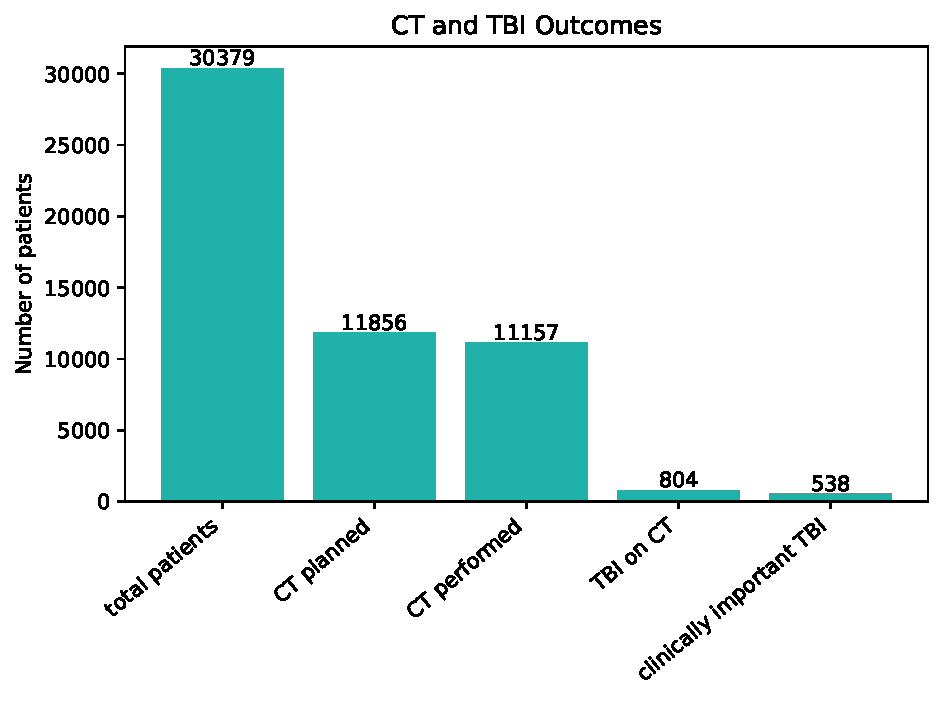
\includegraphics[width=0.8\textwidth]{../figs/ct_tbi_outcomes.pdf}
    \caption{Patient progression through CT and traumatic brain injury (TBI) outcomes.}
\end{figure}

Next, for patients for whom a CT scan was planned, I explored the indicators that influenced
the decision to obtain a CT scan. Specifically, I looked at the five most frequently selected
indicators for two age groups: patients less than two years old and those two years or older (Fig. 2).
Physicians could select more than one indicator per patient. For both age groups, injury mechanism
was the most frequently selected indicator (aside from young age among patients less than two years old).
Vomiting after injury was also in the top five selected indicators both both age groups.

\begin{figure}[H]
    \centering
    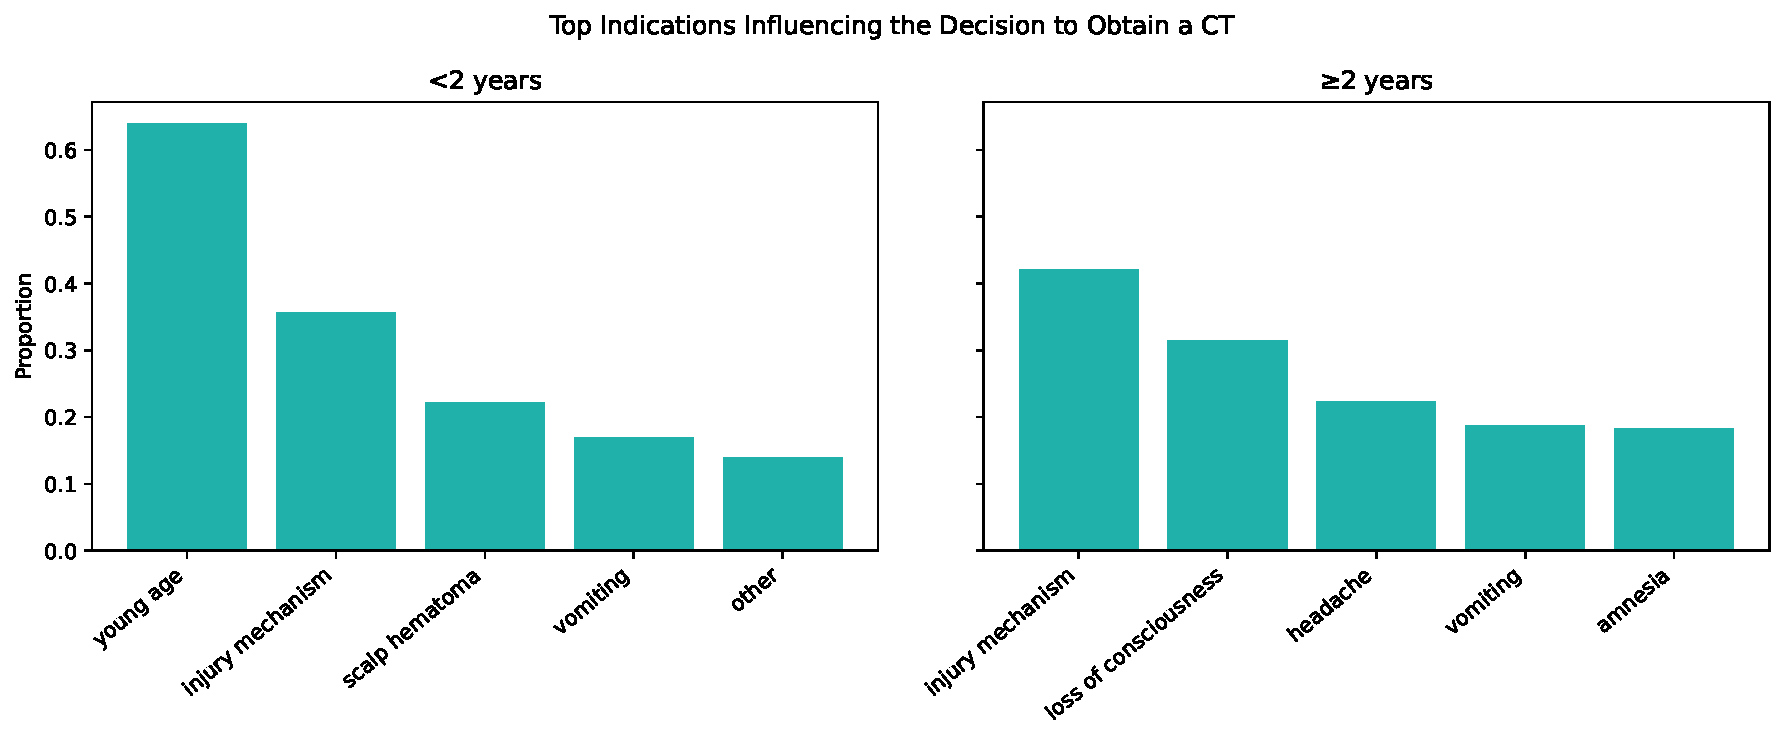
\includegraphics[width=\textwidth]{../figs/top_ct_indicators.pdf}
    \caption{Top indicators influencing the decision to obtain a CT. Only patients for whom a CT scan was planned are included. Physicians could select more than one indicator per patient.}
\end{figure}

Given that injury mechanism was such a frequently selected indicator for both age groups,
I decided to explore it further. Among patients for whom a CT scan was planned and injury mechanism 
was selected as an important indicator, I examined the relative frequency of specific injury mechanisms (Fig. 3).
Fall from elevation and motor vehicle collision were the most common. This seems reasonable, as these 
mechanisms have the potential to result in more serious injuries than some of the other mechanisms 
(such as fall from standing) and are also likely more common than others (such as assault).

\begin{figure}[H]
    \centering
    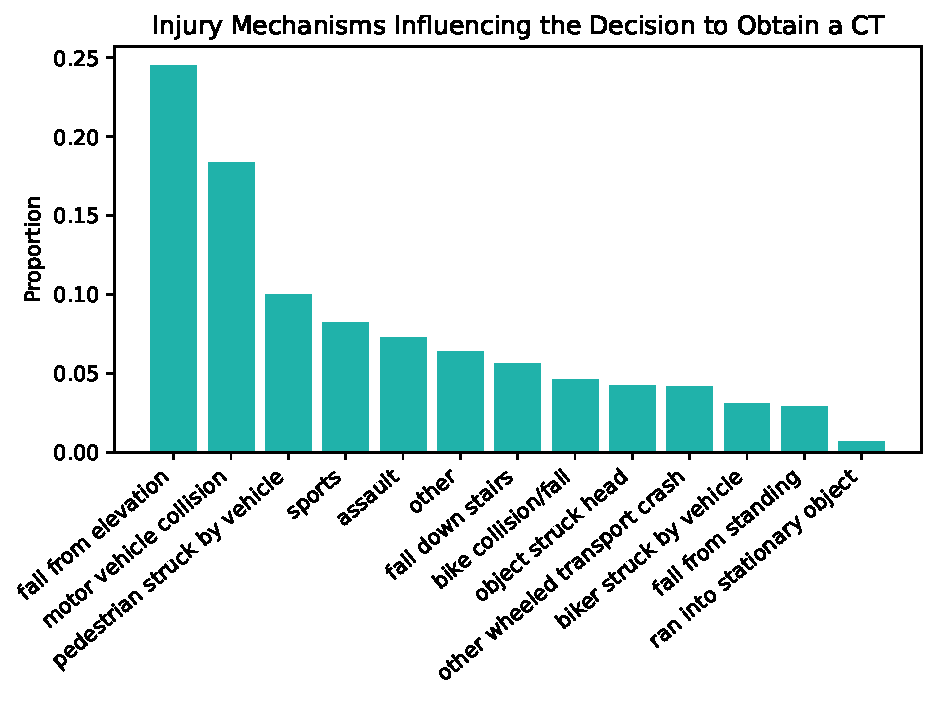
\includegraphics[width=0.8\textwidth]{../figs/injury_mech.pdf}
    \caption{Injury mechanisms influencing the decision to obtain a CT. Only patients for whom a CT scan was planned and injury mechanism was selected as an indicator are included.}
\end{figure}

\section{Findings}\label{findings}

\subsection{First finding}\label{first-finding}

My initial data exploration motivated me to investigate injury mechanisms more closely. 
Additionally, Kuppermann et al. (2009) focus more on injury mechanism severity
than on the mechanism itself, making a distinction between mild or moderate severity and high severity.
This led me to investigate whether (1) there is a substantial difference in ciTBI risk between moderate- and high-
severity injuries and (2) the injury mechanism itself may also be informative of ciTBI risk.

I explored differences in the proportion of patients with ciTBI across injury mechanisms 
that had both moderate- and high-severity cases (Fig. 4). Following Kuppermann et al. (2009), I excluded 
patients with GCS scores less than 14 (for those patients the risk of ciTBI substantially
outweighs the radiation risk from CT). For several mechanisms 
(motor vehicle collision, sports, fall from elevation, other), we see the expected pattern:
high-severity cases have a meaningfully higher proportion of ciTBI than moderate-severity cases.
However, for some mechanisms (object struck head and pedestrian struck by vehicle),
the difference in the proportion of ciTBI between moderate- and high-severity cases is relatively small.
Surprisingly, for a few mechanisms (biker struck by vehicle and assault), the pattern is reversed,
with moderate-severity cases having a higher proportion of ciTBI than high-severity cases.
Furthermore, for both biker and pedestrian struck by vehicle, 
the mechanism itself appears potentially informative of ciTBI risk beyond the assigned mechanism severity,
as both moderate- and high-severity cases have relatively high proportions of ciTBI. 

Overall, this finding suggests that considering certain injury mechanisms, such as being stuck by a vehicle,
in addition to mechanism severity may provide useful information when developing a clinical decision rule.

\begin{figure}[H]
    \centering
    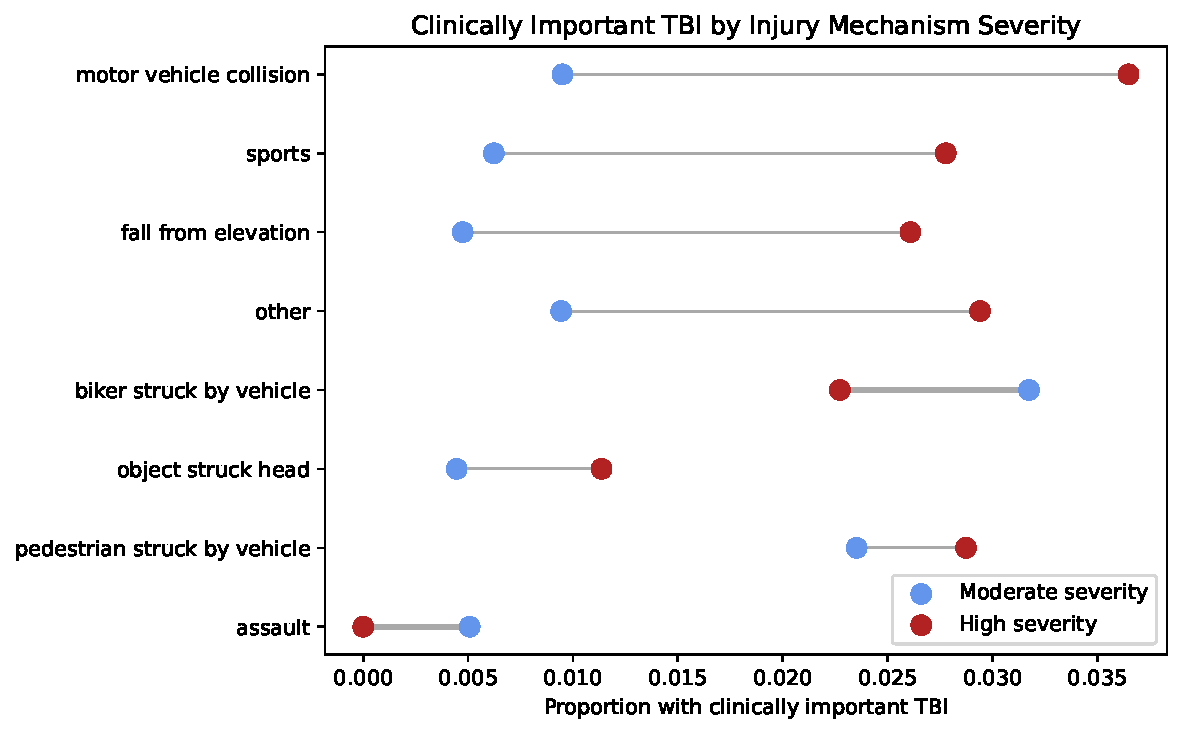
\includegraphics[width=\textwidth]{../figs/injury_mech_severity.pdf}
    \caption{Clinically important TBI by injury mechanism severity. Injury mechanisms are ordered by the difference in the proportion with ciTBI between moderate- and high-severity cases. Only patients with a Glasgow Coma Scale (GCS) score $\geq 14$ are included. A bold line indicates that the proportion with ciTBI was greater for moderate- than high-severity cases.}   
\end{figure}

\subsection{Second finding}\label{second-finding}

The prediction tree and suggested CT algorithm from Kuppermann et al. (2009) ultimately rely largely on 
relatively simple parent or composite variables (e.g., any history of vomiting or any history of loss of consciousness). 
This makes sense since the clinical decision rule needs to be relatively simple and easy to use.
However, it left me curious as to whether some of the more detailed child variables 
might also provide useful information, especially since they make up a substantial portion of the available dataset. 

From my initial data exploration, vomiting after injury was one of the five most frequently selected
indicators influencing the decision to obtain a CT scan for both age groups (Fig. 2). 
This motivated me to investigate some of the child variables associated with vomiting after injury. 
As in the previous finding, I excluded patients with GCS scores less than 14.

For patients two years or older, vomiting within one hour of injury appears to be 
associated with a higher proportion of ciTBI (Fig. 5). The proportion of patients with ciTBI was 
relatively high across this entire column ($>0.02$, or 2.0\%). For patients less than two years old, 
the number of vomiting episodes appears to be potentially informative of ciTBI risk,
with the proportion of ciTBI relatively high across the row representing more than two episodes 
($\geq 0.02$, or 2.0\%). 

This finding suggests that vomiting soon after injury might be an important symptom to 
consider for patients two years or older, whereas multiple vomiting episodes might
provide useful information for patients less than two years old. Interestingly, history of vomiting
was included in the prediction tree and suggested CT algorithm from Kuppermann et al. (2009)
only for patients two years or older. More broadly, this finding suggests that 
certain child variables may provide useful information beyond their parent variables.
However, the increased complexity associated with incorperating these varriables
into a clinical decision rule may not ultimately be worthwhile. 

\begin{figure}[H]
    \centering
    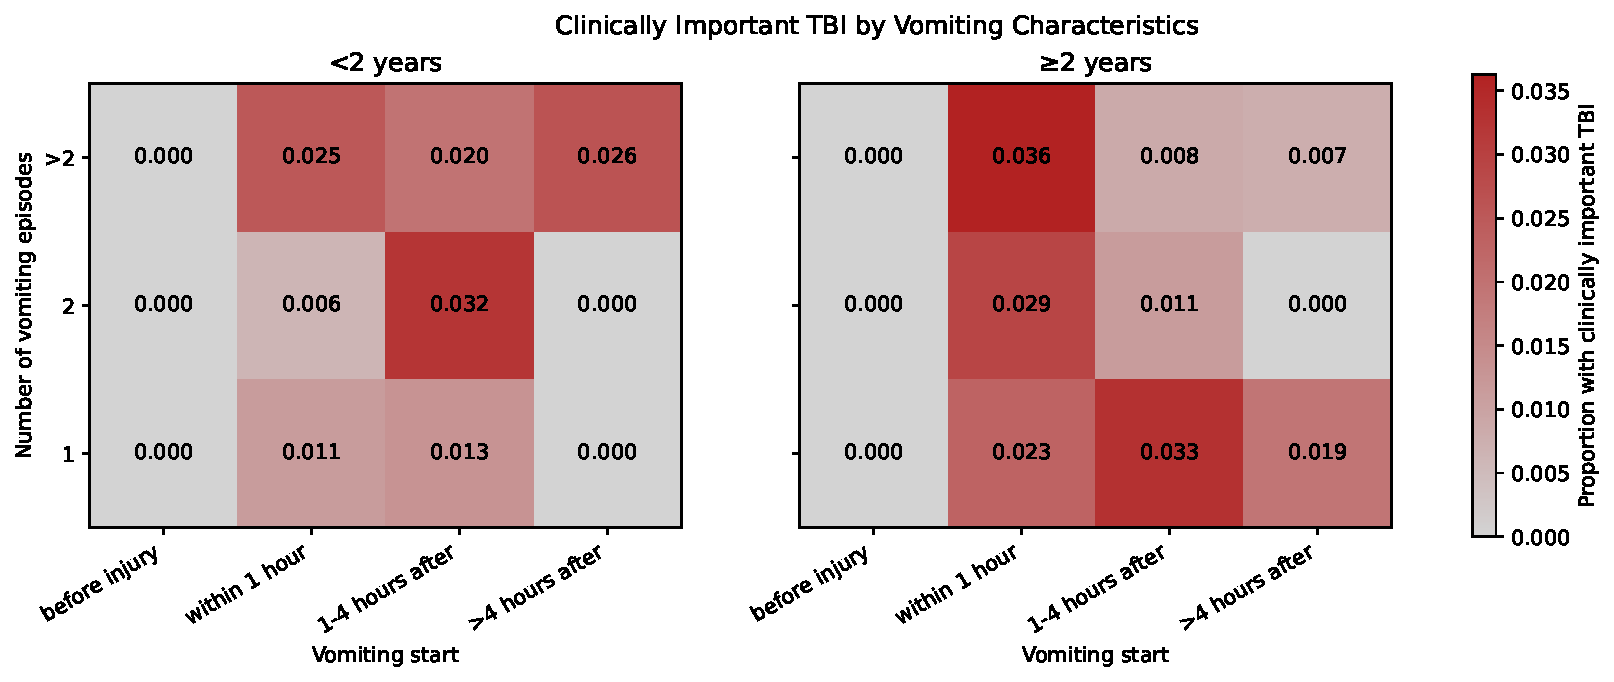
\includegraphics[width=\textwidth]{../figs/vomiting.pdf}
    \caption{Clinically important TBI by vomiting characteristics. Only patients with a history of vomiting and a Glasgow Coma Scale (GCS) score $\geq 14$ are included.}
\end{figure}

\subsection{Reality Check}\label{reality-check}

As a reality check, I compared key summary statistics from my cleaned data with those 
reported in Figure 1 (flow chart) and Table 1 (distribution of prediction rule 
variables and outcomes) of Kuppermann et al. (2009) (Table 1).
I assume that the variables in my dataset correspond to those used to produce the published 
summaries and that, after cleaning and preprocessing, the counts should therefore be reasonably similar. 

Overall, I think my cleaned data generally pass the reality check.
Perfect agreement is not expected given that there are multiple valid 
approaches to cleaning and preprocessing a dataset.
The discrepancy in total number of patients with GCS 14-15 can be explained
by that Kuppermann et al. (2009) excluded 18 patients with missing primary outcomes.
In general, my cleaned counts were slightly higher for the number of vomiting episodes 
and injury mechanism severity than those reported by Kuppermann et al. (2009).
This may be because Kuppermann et al. (2009) did not impute,
or did so less extensively than I did during preprocessing, which 
represents a reasonable difference in data-cleaning approaches. 

\begin{table}[H]
    \centering
    \caption{Reality check comparing patient counts in my cleaned data with those reported by Kuppermann et al. (2009).}
    \begin{tabular}{llrr}
        \toprule
        Variable & Level & Kuppermann & My cleaned data \\
        \midrule
        GCS 14--15 & & 42,412 & 42,430 \\
        ciTBI ($<2$) & & 98 & 98 \\
        ciTBI ($\geq2$) & & 278 & 278 \\
        \midrule
        Number of vomiting episodes ($<2$) & 0 & 9,071 & 9,074 \\
        & 1 & 676 & 684 \\
        & 2 & 308 & 309 \\
        & $>2$ & 512 & 572 \\
        & total & 10,567 & 10,639 \\
        \midrule
        Number of vomiting episodes ($\geq2$) & 0 & 27,484 & 27,497 \\
        & 1 & 1,412 & 1,436 \\
        & 2 & 800 & 800 \\
        & $>2$ & 1,596 & 1,757 \\
        & total & 31,292 & 31,490 \\
        \midrule
        Injury mechanism severity & mild & 7,106 & 7,108 \\
        & moderate & 29,124 & 28,743 \\
        & severe & 5,869 & 6,296 \\
        & total & 42,099 & 42,147 \\
        \bottomrule
    \end{tabular}
\end{table}

\subsection{Stability Check}\label{stability-check}

As a stability check, I chose an alternative way to preprocess truly missing categorical child variables
(i.e., the child variables were not missing because the parent was a 0 (no) or missing).
Originally, I imputed missing child values using the most common combination among
similar cases. This approach used the observed values of one child variable to help
inform the imputation of another child variable, preserving some of the potential relationships
among child variables. Here, I chose the second, simpler option, where I imputed each missing
child variable using its overall mode, without considering the values of the other non-missing child variables. 

For patients two years or older, the overall pattern and takeaway remained stable: 
vomiting within one hour of injury appears to be associated with a higher proportion of ciTBI (Fig. 6).
However, for patients less than two years old, the overall pattern and conclusion were not stable.
Under this perturbation, I would no longer conclude that the number of vomiting episodes is
potentially informative of ciTBI risk. This version potentially aligns more closely with 
Kuppermann et al. (2009), in which history of vomiting was included in the prediction tree 
and suggested CT algorithm only for patients two years or older.

\begin{figure}[H]
    \centering
    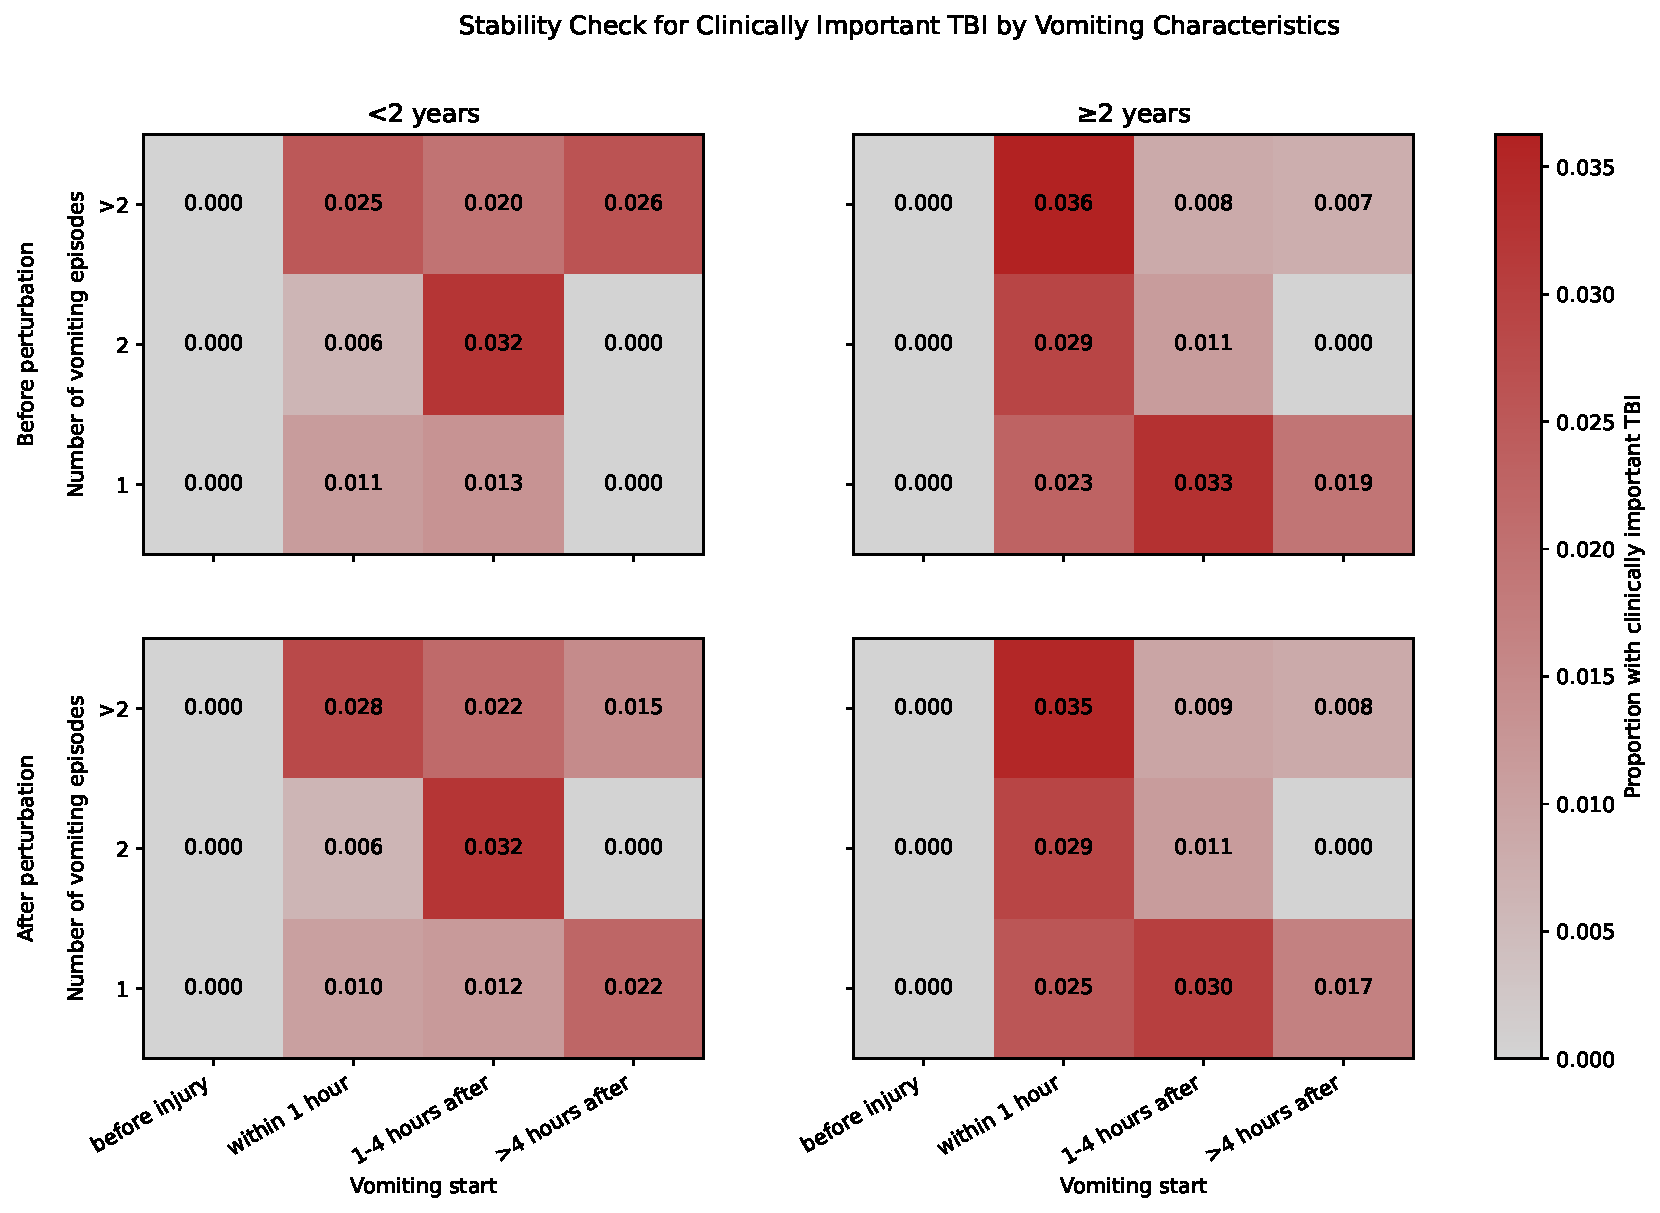
\includegraphics[width=\textwidth]{../figs/vomiting_stability.pdf}
    \caption{Clinically important TBI by vomiting characteristics before and after data preprocessing perturbation. The perturbation involved changing the method used to impute missing categorical child variables.}
\end{figure}

\section{Modeling}

\subsection{Implementation}

I implemented two different classification methods to determine whether or not a CT scan should be recommended. 
For the first method, I applied a modified version of the clinical decision rule from Kuppermann et al. (2009),
including specific variables of interest identified through my exploratory analysis, such as whether a patient was 
struck by a vehicle, vomiting within one hour of injury (for patients two years or older), and
more than two vomiting episodes (for patients less than two years old). 

For the second method, I fit a logistic regression separately for each age group using LogisticRegression from
sklearn with no penalization. I restricted the models to patients with GCS scores $\geq 14$
and used the same predictors as the modified Kuppermann et al. (2009) decision rule. 
I chose a classification threshold that achieved at least 90\% 
sensitivity on the training set to minimize the number of missed diagnoses.  

To evaluate model performance, I calculated sensitivity, specificity, and CT recommendation rate
for the test data. The clinical decision rule should have high sensitivity 
(i.e., a high proportion of patients with ciTBI should have CT recommended) and 
high specificity (i.e., a high proportion of patients without ciTBI should not have CT recommended). 
Although sensitivity is the primary consideration, high specificity is also important
because unnecessary CT scans expose patients to radiation, as previously discussed. 

\subsection{Stability}

I implemented the same stability check of choosing an alternative way to preprocess truly missing categorical child variables.
Model performance was quite stable (Table 2). For the logistic regressions, the coefficients 
were also very stable. As an example, for the logistic regression for patients less than two years old,
the coefficients did not change very much in magnitude and none of them changed sign (Fig. 7). 

\begin{table}[htbp]
    \centering
    \begin{tabular}{lcccccc}
        \hline
        & \multicolumn{2}{c}{Modified Kuppermann} 
        & \multicolumn{2}{c}{Logistic ($<2$)} 
        & \multicolumn{2}{c}{Logistic ($\geq 2$)} \\
        & Before & After
        & Before & After
        & Before & After \\
        \hline
        Sensitivity & 0.936 & 0.936 & 0.900 & 0.900 & 0.892 & 0.892 \\
        Specificity & 0.602 & 0.603 & 0.550 &  0.553 & 0.687 & 0.687 \\
        CT recommendation rate & 40.2 & 40.2 & 45.3 & 45.0 & 31.7 & 31.7 \\
        \hline
    \end{tabular}
    \caption{Model performance metrics before and after data preprocessing perturbation. The perturbation involved changing the method used to impute missing categorical child variables.}
    \label{tab:model_performance}
\end{table}

\begin{figure}[H]
    \centering
    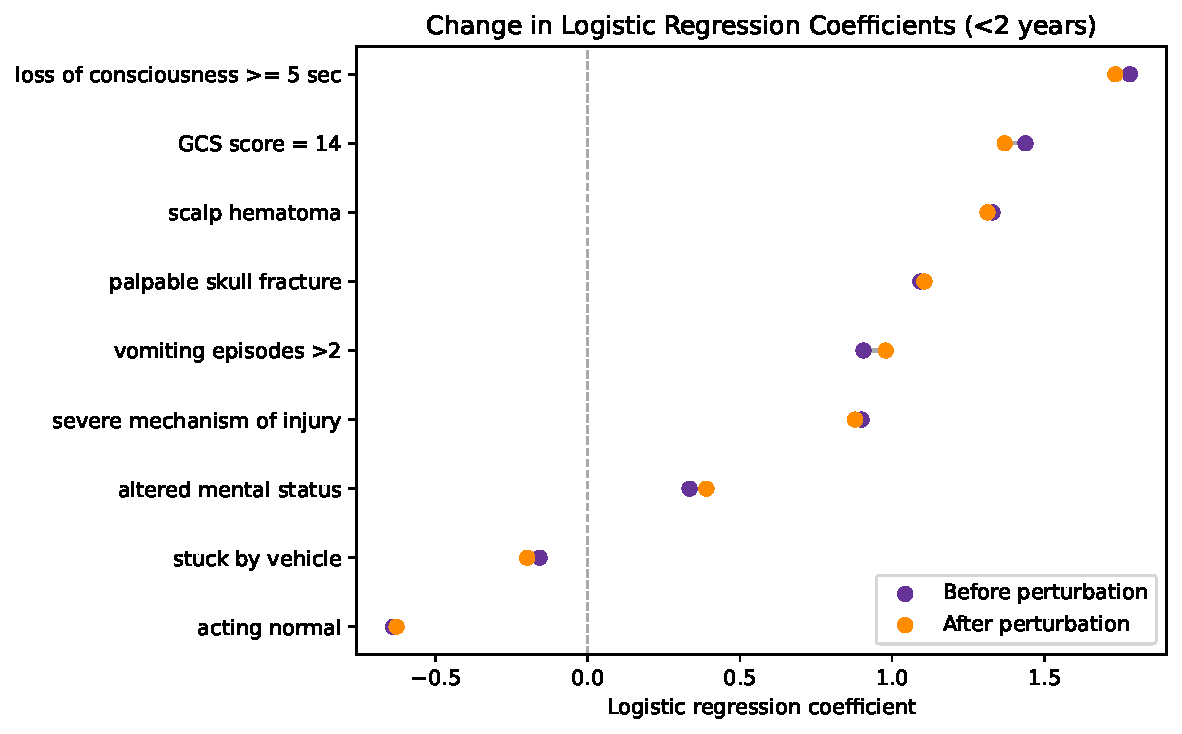
\includegraphics[width=0.9\textwidth]{../figs/log_reg_stability.pdf}
    \caption{Logistic regression coefficients before and after data data preprocessing perturbation. The perturbation involved changing the method used to impute missing categorical child variables.}
\end{figure}

\subsection{Discussion}

The modified Kuppermann et al. (2009) clinical decision rule is certainly in a simple,
interpretable form. However, there is no way to gauge the potential relative importance
of the included variables from the rule itself. 

It would be difficult for a physician to directly use the logistic regression 
by predicting the probability of ciTBI and comparing it to a predetermined 
threshold. However, it could be useful if the physician was able to input the 
patient information into a user interface that returned the model recommendation,
although this is likely less practical in reality. A benefit of the logistic regression 
is that it allows the magnitude and sign of the log-odds coefficients to be 
examined to potentially better understand each variable's association with ciTBI.
For example, loss of consciousness $\geq 5$ seconds has a coefficient around 1.7 (Fig. 7),
indicating that it is associated with a substantial increase in the log-odds of ciTBI, 
holding other predictors constant. 

\section{Conclusion}\label{conclusion}

Veridical data science requires a strong connection between three different realms: reality (the real world where decisions are made),
approximation of reality (where data and future data live), and the mental construct (where algorithms/models live).
The data cleaning, preprocessing, and exploratory analysis steps all help ensure that the data are
a reasonable approximation of reality, although data and reality never have a perfect one-to-one correspondence. 
The stability checks help ensure that conclusions remain fairly consistent under reasonable perturbations, 
which strengthens the connections between reality, data, and future data. The modeling component of 
this lab belongs to the third realm but should remain strongly connected to decisions made in reality. 

Overall, the PECARN data seem strongly connected to reality. It is a useful dataset for addressing the domain
problem of vetting and/or improving the clinical decision rule for ciTBI, especially because 
the variables are all readily available to physicians when they are deciding whether to obtain a CT scan,
strengthening the connection between the data and real-world decisions. The size of the dataset is both 
helpful and challenging. The large number of observations is helpful, while the 
large number of variables makes it somewhat challenging to clean and explore, especially given the 
nested parent/child hierarchy.  

\section{Academic honesty statement}\label{academic-honesty-statement}

Professor Bin Yu, I affirm that the work in this report is my own and sources are properly cited. 
In accordance with class policy, I used ChatGPT 5.6 to look up generic Python how-tos since I am coming from primarily using R, 
debug code, and provide suggestions for particularly tricky pieces. I also used it to help polish some 
of my writing at the paragraph level (to improve awkward wording and identify typos). I reviewed, edited, and
iterated on any code or writing suggestions from ChatGPT. Academic research honesty is necessary for our own learning 
and for maintaining trust within and outside the academic community.

\section{Bibliography}\label{bibliography}

Kuppermann, N., et al. (2009). Identification of children at very low risk of clinically-important brain injuries after head trauma:
a perspective cohort study. Lancet 374:1160-1170.

\end{document}
